\documentclass[11pt]{memoir}
\usepackage[utf8]{inputenc}
 
\usepackage{amsmath}
\usepackage[polutonikogreek,francais,english]{babel}
\usepackage{setspace}
\usepackage{subfig}  
\usepackage{booktabs}
\usepackage{titlesec}
\usepackage{url}
\usepackage{graphicx} 
\usepackage{longtable}
\usepackage{makecell} 
\usepackage{bigdelim}
\usepackage{multirow}
\usepackage{caption}
\captionsetup{font=small}
\usepackage{wrapfig}
\usepackage{braket}
\usepackage{chemfig}
\usepackage{amssymb}
\usepackage{wasysym}
\usepackage[stable]{footmisc}

\usepackage{graphicx}  % provides macros for importing of graphics
%\usepackage{fullpage}  % sets margins to fill out the page (1")
\usepackage{url}       % provides easy URL formatting
\usepackage{amsmath}   % provides mathematics macros
\usepackage{setspace}  % provides macros for manipulating spacing
%\usepackage{floatflt} %
%\usepackage{fancyhdr}  % provides macros for setting running headers, etc
\usepackage{titlesec}  % provides macros for manipulating section formats
\usepackage{wrapfig}   % provides macros for figures to be wrapped by text
%\pagestyle{fancy}
 
%
% Set some global parameters
%
\settrimmedsize{11in}{210mm}{*} 
\setlength{\trimtop}{0pt} 
\setlength{\trimedge}{\stockwidth} 
\addtolength{\trimedge}{-\paperwidth} 
\settypeblocksize{7.75in}{33pc}{*} 
\setulmargins{4cm}{*}{*} 
\setlrmargins{1.25in}{*}{*} 
\setmarginnotes{17pt}{51pt}{\onelineskip} 
\setheadfoot{\onelineskip}{2\onelineskip} 
\setheaderspaces{*}{2\onelineskip}{*} 
\checkandfixthelayout 

\setcounter{secnumdepth}{0} % only the chapters will display numbers
\setcounter{tocdepth}{1}    % only chapters and section will appear in TOC
%
% define places to look for figures so that we don't have to include the directory-name every time
% we refer to a figure
%
\graphicspath{{ }{./fig/}}
%{./chapterI/fig/}{./chapterII/fig/}{./chapterIII/fig/}{./chapterIV/fig/}{./chapterV/fig/}}
%
% Define some math commands
%
\renewcommand{\vec}[1]{\mathbf{#1}}
\newcommand{\dif}[1]{\frac{d}{d #1}}
\newcommand{\Dif}[1]{\frac{\partial}{\partial #1}}
\newcommand{\der}[2]{\frac{d #2}{d #1}}
\newcommand{\Der}[2]{\frac{\partial #2}{\partial #1}}
\newcommand{\dder}[2]{\frac{d^2 #2}{d #1^2}}
\newcommand{\DDer}[2]{\frac{\partial^2 #2}{\partial #1^2}}
\newcommand{\MDer}[3]{\frac{\partial^2 #3}{\partial #1\partial #2}}
\renewcommand{\colon}{\negthinspace :\negthinspace}
\newcommand{\ratio}[2]{#1\negthinspace :\negthinspace #2}
%
% Code below defines a new enumerate environment where spacing between items can be controlled. 
% Used at end of Einstein paper.
\newenvironment{tight_enumerate}{
\begin{enumerate}
  \setlength{\itemsep}{3pt}
  \setlength{\parskip}{0pt}
}{\end{enumerate}}
% End of new enumerate environment

% abbreviations
%
\providecommand{\e}[1]{\ensuremath{\times 10^{#1}}}

\def\etal{{\textsl et al.}}
\def\ie{{\textsl i.e.}}
\def\eg{{e.g.}}
\def\th{{$^{th}$}}
\def\nd{{$^{nd}}}
\def\st{{$^{st}$}}
\def\etc{{\textsl etc.}}
 
\hyphenation{
ab-sorp-tion ac-com-pan-ied a-chieved ag-gre-gate al-ter-na-tive al-though a-nal-o-gy ap-pa-rat-us ap-pli-ca-tion ap-plied ap-pro-pri-ate ap-prox-i-ma-tion ap-prox-i-ma-tions ar-range-ment ar-range-ments as-so-ci-a-tion as-sump-tion at-ten-tion base-ment be-cause be-long be-tween Boltz-mann cal-cu-la-tion ca-ta-stro-phe char-ac-ter char-ac-ter-iz-ing char-ac-ter-is-tic char-ac-ter-ize char-ac-ter-ized chem-i-stry cir-cum-stan-ces clas-si-cal co-in-ci-dence com-bi-na-tion com-pare com-pared com-po-nents com-plete-ly com-pli-ca-ted com-pu-ta-tions con-di-tions con-nect-ed con-nec-tion con-se-quence con-se-quent con-sid-er-a-tion con-sid-ered con-stant con-stants con-struct-ing con-tra-dict cor-pus-cul-ar cor-rel-a-tive-ly cor-re-spond-ing cy-lin-dri-cal deal-ing de-lo-cal-iz-a-tion de-lo-cal-ize de-lo-cal-ized de-scrib-ing de-scrip-tion de-tec-tor de-tec-tors de-ter-mined de-vel-op-ment di-a-phragm dif-fer-end dis-ap-pear dis-ap-pears dis-crim-i-na-tion dis-place-ment dis-cus-sion dis-per-sion dis-sem-i-nates dis-tance dis-tan-ces dis-tin-guish dis-trib-ut-ed e-lec-tro-mag-net-ic e-lec-tron e-lec-trons el-e-ment el-e-men-ta-ry e-mit-ted en-er-gy en-er-gies en-tire-ly en-vi-ron-ment e-qua-tion e-qui-lib-ri-um e-qui-par-ti-tion e-ven-tu-al-i-ty ex-cep-tion-al ex-chang-es ex-ist-ence ex-pe-ri-en-ces ex-pe-ri-ence ex-per-i-ment ex-per-i-ments ex-per-i-men-tal ex-per-i-ment-al-ly ex-plains ex-pla-na-tion ex-po-nen-tial ex-po-nen-tials ex-press-es ex-treme-ly fluc-tu-a-tions fol-low-ing for-mu-lat-ed for-mu-late foun-da-tion fre-quen-cies fre-quen-cy fun-da-men-tal ge-o-met-ric-al ge-o-met-ric-al-ly grav-i-ta-tion-al guid-ing har-mon-ics Heis-en-berg ho-mo-ge-ne-ous hy-dro-gen hy-poth-e-sis im-por-tant in-can-des-cent in-com-plete in-creas-ing in-deed in-de-pen-dent in-de-ter-mi-nate in-de-ter-min-a-cy in-e-qual-i-ty in-for-ma-tion in-stru-ment in-stru-ments in-ter-ac-tion in-ter-est-ed in-ter-fer-ence in-ter-fer-om-e-ter in-ter-mo-lec-u-lar in-ter-pre-ta-tion in-tro-duc-ing in-ves-ti-gate in-volves la-bo-ra-to-ry lo-cal-ize lo-cal-ized math-e-mat-ics math-e-mat-i-cal Mau-per-tuis Max-wel-li-an me-chan-i-cal me-chan-ics mean-ing-less meas-ure-ment meas-ure-ment meas-ure-ments mol-e-cules mo-men-tum nev-er-the-less nu-mer-ous ob-jec-tion ob-jec-tions ob-ser-va-tion ob-serv-a-ble ob-serv-a-bles ob-served par-tic-u-lar par-tic-u-lar-ly par-tic-u-lars per-mit-ting per-pen-dic-u-lar phe-nom-e-na pho-to-di-ode pho-to-di-odes pho-to-e-lec-tric pho-to-graph-ic pho-to-lu-mi-nes-cence phys-i-cal phy-si-cists pol-ar-i-za-tion pol-a-rize pol-a-rized pol-a-riz-er pol-a-riz-ers pos-si-bil-i-ties pos-si-bil-i-ty po-ten-tial pre-cis-ion pre-dic-tion prin-ci-ple pro-ced-ure pro-duce pro-duced pro-per-ties pro-per-ty pro-por-tion-al pro-vid-ed quan-ti-ta-tive quan-ti-ties quan-ti-za-tion quant-um ques-tion ques-tions ra-di-a-tion re-cog-ni-tion re-pre-sen-ta-tion re-flect-ed re-gard-ing re-placed re-quest-ed ri-gid-ly Ruth-er-ford sche-mat-ic-al-ly sep-a-rate sep-a-rat-ed sim-pli-fi-ca-tion si-mul-ta-ne-ous sit-u-a-tion some-what Som-mer-feld spec-trom-e-ter spec-tro-scop-ic spec-trum stand-ard stand-ing some-thing struc-ture sub-stan-ces sub-trac-tions suc-ces-sive su-per-po-si-tion sup-posed sur-round-ing sur-round-ings tem-per-a-ture the-o-ret-i-cal ther-mal trans-mit-ted treat-ment un-der-stand-ing Thom-son un-a-void-a-bly un-der-stand-a-ble un-found-ed Un-ge-nau-ig-keit-en un-pre-dict-a-ble var-i-a-ble 
}


\chapterstyle{thatcher}
\renewcommand{\chaptitlefont}{\normalfont\scshape\huge}

\renewcommand{\rmdefault}{ppl}
\renewcommand{\sfdefault}{phv}
\renewcommand{\ttdefault}{pcr}

\title{The Completeness of Quantum Mechanics and the Locality Principle}

\begin{document}
\section*{The Completeness of Quantum Mechanics and the Locality Principle}

This chapter presents Einstein's objections to the Copenhagen
interpretation of wave mechanics and Bohr's response, followed by David
Bohm's interesting interpretation of the implications of Einstein's
argument. Einstein presented his objections in the form of various
thought-experiments. The most probing of these appears in a paper ``Can
Quantum-Mechanical Description of Reality be Considered Complete?'' by
Einstein, Podolsky, and Rosen (referred to as EPR), which is still the
object of debate among physicists and philosophers.

In discussions with Bohr and others over a period of years, Einstein had
tried to devise a thought-experiment that would demonstrate the
incompleteness of wave mechanics. Bohr offers the following summary of
these conversations:

\subsection*{Niels Bohr: Einstein's Objections to Quantum Mechanics\footnote{From
  ``Discussion with Einstein on Epistemological Problems in Atomic
  Physics,'' in P.A. Schilpp, ed., \emph{Albert Einstein:
  Philosopher-Scientist} (Evanston: The Library of Living Philosophers,
  1949), 208-17. Reprinted in J. Wheeler and W. Zurek, eds.,
  \emph{Quantum Theory and Measurement} (Princeton University Press,
  1983), 19-26. Hereafter the latter work will be referred to as
  \emph{QTM}. Changes in notation will be made occasionally.}}


\begin{quote}
To illustrate his attitude, Einstein referred at one of the
sessions to the simple example, illustrated by Figure 1 of a particle
(electron or photon) penetrating through a hole or a narrow slit in a
diaphragm placed at some distance before a photographic plate. On
account of the diffraction of the wave connected with the motion of the
particle 
%
\begin{figure}[h] % Figure 1
  \begin{center}
    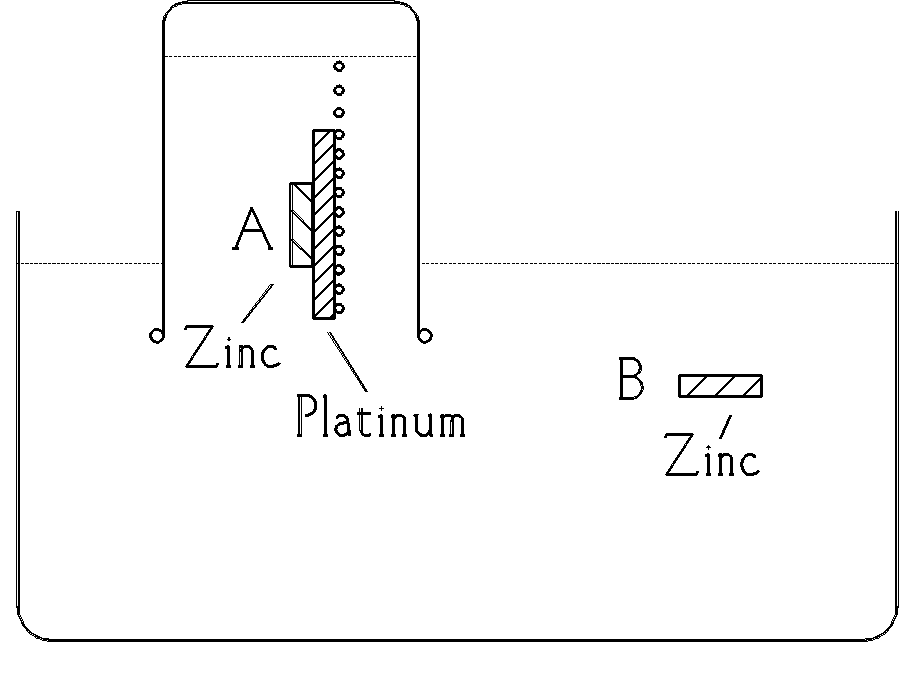
\includegraphics[width=2.82293in,height=2.09933in]{images/18_epr/image001.png}
  \end{center}
\end{figure}
%
and indicated in the figure by the thin lines, it is under such
conditions not possible to predict with certainty at what point the
electron will arrive at the photographic plate, but only to calculate
the probability that, in an experiment, the electron will be found
within any given region of the plate. The apparent difficulty, in this
description, which Einstein felt so acutely, is the fact that, if in the
experiment the electron is recorded at one point A of the plate, then it
is out of the question of ever observing an effect of this electron at
another point (B), although the laws of ordinary wave propagation offer
no room for a correlation between two such events.

Einstein's attitude gave rise to ardent discussions within a small
circle\ldots{} The discussions, however, centered on the question of
whether the quant\-um-me\-chan\-i\-cal description exhausted the possibilities
of accounting for observable phenomena or, as Einstein maintained, the
analysis could be carried further and, especially, of whether a fuller
description of the phenomena could be obtained by bringing into
consideration the detailed balance of energy and momentum in individual
processes\ldots.

The problem raised by Einstein was now to what extent a
control\footnote{{[}``a control'': Here meaning \emph{an ascertainment}
  or \emph{a verification}. Compare Schrödinger's similar usage in
  Chapter IX, 162 above.{]}} of the momentum and energy transfer,
involved in a location of the particle in space and time, can be used
for a further specification of the state of the particle after passing
through the hole. Here, it must be taken into consideration that the
position and the motion of the diaphragm and the shutter have so far
been assumed to be accurately coordinated with the space-time reference
frame. This assumption implies, in the description of the state of these
bodies, an essential latitude as to their momentum and energy which need
not, of course, noticeably affect the velocities, if the diaphragm and
the shutter are sufficiently heavy. However, as soon as we want to know
the momentum and energy of these parts of the measuring arrangement with
an accuracy sufficient to control the momentum and energy exchange with
the particle under investigation, we shall, in accordance with the
general indeterminacy relations, lose the possibility of their accurate
location in space and time. We have, therefore, to examine how far this
circumstance will affect the intended use of the whole arrangement and,
as we shall see, this crucial point clearly brings out the complementary
character of the phenomena.

Returning for a moment to the case of the simple arrangement indicated
in Figure 1, it has so far not been specified to what use it is
intended. In fact, it is only on the assumption that the diaphragm and
the plate have well-defined positions in space that it is impossible,
within the frame of the quantum-mechanical formalism, to make more
detailed predictions as to the point of the photographic plate where the
particle will be recorded. If, however, we admit a sufficiently large
latitude in the knowledge of the position of the diaphragm it should, in
principle, be possible to control the momentum transfer to the diaphragm
and, thus, to make more detailed predictions as to the direction of the
electron path from the hole to the recording point. As regards the
quantum-mechanical description, we have to deal here with a two-body
system consisting of the diaphragm as well as of the particle, and it is
just with an explicit application of conservation laws to such a system
that we are concerned in the Compton effect\footnote{{[}See n. 15 in
  Chapter X.{]}} where, for instance, the observation of the recoil of
the electron by means of a cloud chamber allows us to predict in what
direction the scattered photon will eventually be observed.

%
\begin{figure}[h] % Figure 2
  \begin{center}
    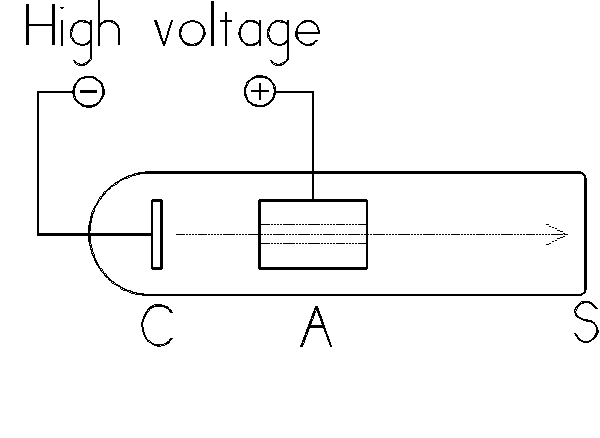
\includegraphics[width=3.78in,height=2.22in]{images/18_epr/image003.png}
  \end{center}
\end{figure}
%


The importance of considerations of this kind was, in the course of the
discussions, most interestingly illuminated by the examination of an
arrangement where between the diaphragm with the slit and the
photographic plate is inserted another diaphragm with two parallel
slits, as is shown in Figure 2. If a parallel beam of electrons (or
photons) falls from the left on the first diaphragm, we shall, under
usual conditions, observe on the plate an interference pattern indicated
by the shading of the photographic plate shown in front view to the
right of the figure. With intense beams, this pattern is built up by the
accumulation of a large number of individual processes, each giving rise
to a small spot on the photographic plate, and the distribution of these
spots follows a simple law derivable from the wave analysis. The same
distribution should also be found in the statistical account of many
experiments performed with beams so faint that in a single exposure only
one electron (or photon) will arrive at the photographic plate at some
spot shown in the figure as a small star. Since now as indicated by the
broken arrows, the momentum transferred to the first diaphragm ought to
be different if the electron was assumed to pass through the upper or
the lower slit in the second diaphragm, Einstein suggested that a
control of the momentum transfer would permit a closer analysis of the
phenomenon and, in particular, to decide through which of the two slits
the electron had passed before arriving at the plate.

A closer examination showed, however, that the suggested control of the
momentum transfer would involve a latitude in the knowledge of the
position of the diaphragm which would exclude appearance of the
interference phenomena in question.\\
\centerline{* * *}
%
\end{quote}

In direct response to EPR, Bohr wrote the following article.


\section*{Can Quantum-Mechanical Description of Physical Reality be Considered
Complete?\footnote{[Bohr's reply to the EPR paper. \emph{Physical
  Review} 48 (1935), 696-702, reprinted in \emph{QTM}, 145-51.]}\\
  {\large N. Bohr}}

{[}The{]} argumentation {[}of Einstein, Podolsky, and Rosen{]} would
hardly seem suited to affect the soundness of quantum-mechanical
description, which is based on a coherent mathematical formalism
covering automatically any procedure of measurement like that indicated.
The apparent contradiction in fact discloses only an essential
inadequacy of the customary viewpoint of natural philosophy for a
rational account of physical phenomena of the type with which we are
concerned in quantum mechanics. Indeed the \emph{finite interaction
between object and measuring agencies} conditioned by the very existence
of the quantum of action entails---because of the impossibility of
controlling the reaction of the object on the measuring instruments if
these are to serve their purpose---the necessity of a final renunciation
of the classical ideal of causality and a radical revision of our
attitude towards the problem of physical reality. In fact, as we shall
see, a criterion of reality like that proposed by the named authors
contains---however cautious its formulation may appear---an essential
ambiguity when it is applied to the actual problems with which we are
here concerned. In order to make the argument to this end as clear as
possible, I shall first consider in some detail a few simple examples of
measuring arrangements.

Let us begin with the simple case of a particle passing through a slit
in a diaphragm, which may form part of some more or less complicated
experimental arrangement. Even if the momentum of this particle is
completely known before it impinges on the diaphragm, the diffraction by
the slit of the plane wave giving the symbolic representation of its
state will imply an uncertainty in the momentum of the particle, after
it has passed the diaphragm, which is the greater the narrower the slit.
Now the width of the slit, at any rate if it is still large compared
with the wave-length, may be taken as the uncertainty $\Delta x$ of the
position of the particle relative to the diaphragm, in a direction
perpendicular to the slit. Moreover, it is simply seen from de Broglie's
relation between momentum and wave-length that the uncertainty $\Delta p$
of the momentum of the particle in this direction is correlated to
$\Delta x$ by means of Heisenberg's general principle $\Delta p\Delta x \approx h$
\ldots. Obviously the uncertainty $\Delta p$ is inseparably
connected with the possibility of an exchange of momentum between the
particle and the diaphragm; and the question of principal interest for
our discussion is now to what extent the momentum thus exchanged can be
taken into account in the description of the phenomenon to be studied by
the experimental arrangement concerned, of which the passing of the
particle through the slit may be considered as the initial stage. Let us
first assume that, corresponding to usual experiments on the remarkable
phenomena of electron diffraction, the diaphragm, like the other parts
of the apparatus---say a second diaphragm with several slits parallel to
the first and a photographic plate---is rigidly fixed to a support which
defines the space frame of reference. Then the momentum exchanged
between the particle and the diaphragm will, together with the reaction
of the particle on the other bodies, pass into this common support, and
we have thus voluntarily cut ourselves off from any possibility of
taking these reactions separately into account in predictions regarding
the final result of the experiment---say the position of the spot
produced by the particle on the photographic plate. The impossibility of
a closer analysis of the reactions between the particle and the
measuring instrument is indeed no peculiarity of the experimental
procedure described, but is rather an essential property of any
arrangement suited to the study of the phenomena of the type concerned,
where we have to do with a feature of \emph{individuality} completely
foreign to classical physics. In fact, any possibility of taking into
account the momentum exchanged between the particle and the separate
parts of the apparatus would at once permit us to draw conclusions
regarding the ``course'' of such phenomena---say through what particular
slit of the second diaphragm the particle passes on its way to the
photographic plate---which would be quite incompatible with the fact
that the probability of the particle reaching a given element of area on
this plate is determined not by the presence of any particular slit, but
by the positions of all the slits of the second diaphragm within reach
of the associated wave diffracted from the slit of the first diaphragm.

By another experimental arrangement, where the first diaphragm is not
rigidly connected with the other parts of the apparatus, it would at
least in principle be possible to measure its momentum with any desired
accuracy before and after the passage of the particle, and thus to
predict the momentum of the latter after it has passed through the slit.
In fact, such measurements of momentum require only an unambiguous
application of the classical law of conservation of momentum, applied
for instance to a collision process between the diaphragm and some test
body, the momentum of which is suitably controlled before and after the
collision. It is true that such a control will essentially depend on an
examination of the space-time course of some process to which the ideas
of classical mechanics can be applied; if, however, all spatial
dimensions and time intervals are taken sufficiently large, this
involves clearly no limitation as regards the accurate control of the
momentum of the test bodies, but only a renunciation as regards the
accuracy of the control of their space-time coordination. This last
circumstance is in fact quite analogous to the renunciation of the
control of the momentum of the fixed diaphragm in the experimental
arrangement discussed above, and depends in the last resort on the claim
of a purely classical account of the measuring apparatus, which implies
the necessity of allowing a latitude corresponding to the
quantum-mechanical uncertainty relations in our description of their
behavior.

The principal difference between the two experimental arrangements under
consideration is, however, that in the arrangement suited for the
control of the momentum of the first diaphragm, this body can no longer
be used as a measuring instrument for the same purpose as in the
previous case, but must, as regards its position relative to the rest of
the apparatus, be treated, like the particle traversing the slit, as an
object of investigation, in the sense that the quantum-mechanical
uncertainty relations regarding its position and momentum must be taken
explicitly into account. In fact, even if we knew the position of the
diaphragm relative to the space frame before the first measurement of
its momentum, and even though its position after the last measurement
can be accurately fixed, we lose, on account of the uncontrollable
displacement of the diaphragm during each collision process with the
test bodies, the knowledge of its position when the particle passed
through the slit. The whole arrangement is therefore obviously unsuited
to study the same kind of phenomena as in the previous case. In
particular it may be shown that, if the momentum of the diaphragm is
measured with an accuracy sufficient for allowing definite conclusions
regarding the passage of the particle through some selected slit of the
second diaphragm, then even the minimum uncertainty of the position of
the first diaphragm compatible with such a knowledge will imply the
total wiping out of any interference effect---regarding the zones of
permitted impact of the particle on the photographic plate---to which
the presence of more than one slit in the second diaphragm would give
rise in case the positions of all apparatus are fixed relative to each
other.

In an arrangement suited for measurements of the momentum of the first
diaphragm, it is further clear that even if we have measured this
momentum before the passage of the particle through the slit, we are
after this passage still left with a \emph{free choice} whether we wish
to know the momentum of the particle or its initial position relative to
the rest of the apparatus. In the first eventuality we need only to make
a second determination of the momentum of the diaphragm, leaving unknown
forever its exact position when the particle passed. In the second
eventuality we need only to determine its position relative to the space
frame with the inevitable loss of the knowledge of the momentum
exchanged between the diaphragm and the particle. If the diaphragm is
sufficiently massive in comparison with the particle, we may even
arrange the procedure of measurements in such a way that the diaphragm
after the first determination of its momentum will remain at rest in
some unknown position relative to the other parts of the apparatus, and
the subsequent fixation of this position may therefore simply consist in
establishing a rigid connection between the diaphragm and the common
support.

My main purpose in repeating these simple, and in substance well-known
considerations, is to emphasize that in the phenomena concerned we are
not dealing with an incomplete description characterized by the
arbitrary picking out of different elements of physical reality at the
cost of {[}sacrificing{]} other such elements, but with a rational
discrimination between essentially different experimental arrangements
and procedures which are suited either for an unambiguous use of the
idea of space location, or for a legitimate application of the
conservation theorem of momentum. Any remaining appearance of
arbitrariness concerns merely our freedom of handling the measuring
instruments, characteristic of the very idea of experiment. In fact, the
renunciation in each experimental arrangement of the one or the other of
two aspects of the description of physical phenomena---the combination
of which characterizes the method of classical physics, and which
therefore in this sense may be considered as complementary to one
another---depends essentially on the impossibility, in the field of
quantum theory, of accurately controlling the reaction of the object on
the measuring instruments, i.e., the transfer of momentum in case of
position measurements, and the displacement in case of momentum
measurements. Just in this last respect any comparison between quantum
mechanics and ordinary statistical mechanics, however useful it may be
for the formal presentation of the theory, is essentially irrelevant.
Indeed we have in each experimental arrangement suited for the study of
proper quantum phenomena not merely to do with an ignorance of the value
of certain physical quantities, but with the impossibility of defining
these quantities in an unambiguous way.

The last remarks apply equally well to the special problem treated by
Einstein, Podolsky and Rosen, \ldots which does not actually involve any
greater intricacies than the simple examples discussed above. The
particular quantum-mechanical state of two free particles, for which
they give an explicit mathematical expression, may be reproduced, at
least in principle, by a simple experimental arrangement, comprising a
rigid diaphragm with two parallel slits, which are very narrow compared
with their separation, and through each of which one particle with given
initial momentum passes independently of the other. If the momentum of
this diaphragm is measured accurately before as well as after the
passing of the particles, we shall in fact know the sum of the
components perpendicular to the slits of the momenta of the two escaping
particles, as well as the difference of their initial positional
coordinates in the same direction; while of course the \ldots{}
difference of the components of their momenta, and the sum of their
positional coordinates, are entirely unknown. In this arrangement, it is
therefore clear that a subsequent single measurement either of the
position or of the momentum of one of the particles will automatically
determine the position or momentum, respectively, of the other particle
with any desired accuracy; at least if the wave-length corresponding to
the free motion of each particle is sufficiently short compared with the
width of the slits. As pointed out by the named authors, we are
therefore faced at this stage with a completely free choice whether we
want to determine the one or the other of the latter quantities by a
process which does not directly interfere with the particle concerned.

Like the above simple case of the choice between the experimental
procedures suited for the prediction of the position or the momentum of
a single particle which has passed through a slit in a diaphragm, we
are, in the ``freedom of choice'' offered by the last arrangement, just
concerned with a \emph{discrimination between different}
\emph{experimental procedures which allow of the unambiguous use of
complementary classical concepts.} In fact to measure the position of
one of the particles can mean nothing else than to establish a
correlation between its behavior and some instrument rigidly fixed to
the support which defines the space frame of reference. Under the
experimental conditions described such a measurement will therefore also
provide us with the knowledge of the location, otherwise completely
unknown, of the diaphragm with respect to this space frame when the
particles passed through the slits. Indeed, only in this way we obtain a
basis for conclusions about the initial position of the other particle
relative to the rest of the apparatus. By allowing an essentially
uncontrollable momentum to pass from the first particle into the
mentioned support, however, we have by this procedure cut ourselves off
from any future possibility of applying the law of conservation of
momentum to the system consisting of the diaphragm and the two particles
and therefore have lost our only basis for an unambiguous application of
the idea of momentum in predictions regarding the behavior of the second
particle. Conversely, if we choose to measure the momentum of one of the
particles, we lose through the uncontrollable displacement inevitable in
such a measurement any possibility of deducing from the behavior of this
particle the position of the diaphragm relative to the rest of the
apparatus, and have thus no basis whatever for predictions regarding the
location of the other particle.

\footnote{{[}This paragraph has been moved from its place in the
  original, which was marred by a type-setting error.{]}}From our point
of view we now see that the wording of the above-mentioned criterion of
physical reality proposed by Einstein, Podolsky and Rosen contains an
ambiguity as regards the meaning of the expression ``without in any way
disturbing a system.'' Of course there is in a case like that just
considered no question of a mechanical disturbance of the system under
investigation during the last critical stage of the measuring procedure.
But even at this stage there is essentially the question of an
\emph{influence} \emph{on the very conditions which define the possible}
\emph{types of predictions regarding the future behavior of the system}.
Since these conditions constitute an inherent element of the description
of any phenomenon to which the term ``physical reality'' can be properly
attached, we see that the argumentation of the mentioned authors does
not justify their conclusion that quantum-mechanical description is
essentially incomplete. On the contrary this description, as appears
from the preceding discussion, may be characterized as a rational
utilization of all possibilities of unambiguous interpretation of
measurements, compatible with the finite and uncontrollable interaction
between the objects and the measuring instruments in the field of
quantum theory. In fact, it is only the mutual exclusion of any two
experimental procedures, permitting the unambiguous definition of
complementary physical quantities, which provides room for new physical
laws, the coexistence of which might at first sight appear
irreconcilable with the basic principles of science. It is just this
entirely new situation as regards the description of physical phenomena,
that the notion of \emph{complementarity} aims at characterizing.\\
%
\centerline{* * *}
%
Th{[}e{]} necessity of discriminating in each experimental arrangement
between those parts of the physical system considered which are to be
treated as measuring instruments and those which constitute the objects
under investigation may indeed be said to form a \emph{principal}
\emph{distinction} \emph{between classical and quantum-mechanical
description of physical phenomena.} It is true that the place within
each measuring procedure where this discrimination is made is in both
cases largely a matter of convenience. While, however, in classical
physics the distinction between object and measuring agencies does not
entail any difference in the character of the description of the
phenomena concerned, its fundamental importance in quantum theory, as we
have seen, has its root in the indispensable use of classical concepts
in the interpretation of all proper measurements, even though the
classical theories do not suffice in accounting for the new types of
regularities with which we are concerned in atomic physics.\\
\centerline{* * *}
%
\section*{Another Interpretation of the EPR Argument}

Bohr's response did not induce Einstein to change his interpretation of
quantum mechanics. He continued to think that, while it might give the
correct statistical laws, it involved an inadequate conception of
individual elementary processes. Thus, he saw it as a provisional theory
that would eventually be superseded because it was based on the wrong
concepts, that is, on ones that did not correspond to the real physical
states. He may have been thinking that concepts such as potential energy
and material point that quantum mechanics inherited from classical
mechanics had to be replaced before physics could go beyond the
statistical laws of quantum theory. Then Einstein would have been using
the EPR argument to try to induce physicists to join him in the search
for radically new physical concepts.

However, Einstein did agree with at least one aspect of Bohr's reply,
namely, his emphasis on the central role of the expression ``without in
any way disturbing a system'' in the EPR argument. This phrase refers to
the assumption that ``no real change can take place in the second system
in consequence of anything that may be done to the first system.'' This
assumption is one formulation of what has become known as the
\emph{locality principle}. In EPR's statement of the argument, it is not
emphasized that this is the major assumption from which the conclusion
follows. This lack of clarity in the presentation of the argument may
have been due to Podolsky, who actually wrote the paper. For Einstein
himself believed that the truth of the locality principle was what
forced the conclusion that quantum mechanics was incomplete.

According to Einstein the ``orthodox'' quantum theoreticians argue as
follows:\footnote{P. Schilpp, ed., \emph{Albert Einstein:
  Philosopher-Scientist} (Open Court, 1970), 681-82. Einstein's symbols
  have been changed.}

\begin{quote}
If the partial systems I and II {[}for example, in the
thought-experiment of the EPR paper{]} form a total system which is
described by its $\psi$-function\ldots. , there is no reason why any mutually
independent existence (state of reality) should be ascribed to the
partial systems I and II viewed separately, \emph{not even if the
partial systems are spatially separated from each other at the
particular time under consideration}. The assertion that, in this latter
case, the real situation of II could not be (directly) influenced by any
measurement taken on I is, therefore, within the framework of quantum
theory, unfounded and (as the paradox {[}that is, the EPR argument{]}
shows) unacceptable.

By this way of looking at the matter it becomes evident that the paradox
forces us to relinquish one of the following two assertions:

(1) the description by means of the $\psi$-function is \emph{complete},

(2) the real states of spatially separated objects are independent of
each other.

On the other hand, it is possible to adhere to (2), if one regards the
$\psi$-function as the description of a (statistical) ensemble of systems
(and therefore relinquishes (1)). However, this view blasts the
framework of the ``orthodox quantum theory.''
\end{quote}

Now, Einstein believed that the locality principle was true. For it
seemed to him that if one were to say that the locality principle is
false, one would have to accept either a kind of causal influence (from
system I to system II) unknown to current physical theories or a signal
(from system I to system II) that traveled faster than the speed of
light. However, in his special theory of relativity, Einstein had shown
that the speed of light was the fastest speed with which a signal could
be transmitted. Thus, Einstein relinquished assertion (1).

Bohr, on the other hand, in his response argued that the real physical
state of system II was not independent of the experimental arrangement
that was set up to measure some quantity of system I. Thus, he was not
forced to abandon the completeness of quantum mechanics.

However, given the argument as Einstein stated it above, there is
another possibility. For one might relinquish both of the assertions and
hold both that quantum mechanics is incomplete \emph{and} that all
things are interconnected. This position was developed by David Bohm.

As opposed to Einstein, Bohm accepted the dynamical concepts with which
quantum mechanics operates, but he supplemented them with new variables
standing for aspects of reality not taken into account by quantum
mechanics. For this reason such a development of quantum theory is known
as a \emph{hidden variables} theory. Bohm claimed that the non-locality
involved neither conflicts with special relativity nor is attributable
to an influence of the experimental apparatus ``on the very conditions
which define the possible types of predictions regarding the future
behavior of the system.''

Bohm agreed with the position on non-locality which Heisenberg had
formulated several years before the EPR paper. Heisenberg thought that
quantum mechanics involved a propagation at a speed greater than the
speed of light but that this did not conflict with special relativity.
Consider an experiment like a double slit experiment where, however,
only one particle (in this case a photon) is directed at the slits. If
there is no photographic plate, the wave function $\psi$ has two parts, one
corresponding to each slit; and they are each non-zero. But if a
photographic plate is introduced near one slit and registers the photon,
then the part of the wave function corresponding to the other slit

\begin{quote}
immediately becomes zero. The experiment at the position of the {[}first
slit{]} thus exerts a kind of action {[}reduction of the wave packet{]}
at the distant {[}region near the second slit{]}, and one sees that this
action is propagated with a velocity greater than that of light.
However, it is also obvious that this kind of action can never be
utilized for the transmission of signals so that it is not in conflict
with the postulates of the theory of relativity.\footnote{{[}From W.
  Heisenberg, \emph{The Physical Principles of the Quantum Theory}
  (University of Chicago Press, 1930), 39.{]}}
\end{quote}

Bohm based his interpretation on his 1952 article in which he had
refuted objections made in 1927 to de Broglie's pilot wave theory. Bohm
had devoted the major portion of that article to the development of a
consistent non-local theory of hidden variables which was able to
reproduce the predictions of quantum mechanics. He later formulated his
interpretation in less technical terms as follows:

\begin{quote}
2. General Considerations on the Sub-Quantum Mechanical Level\footnote{{[}From
  D. Bohm, \emph{Causality and Chance in Modern Physics} (Philadelphia:
  University of Pennsylvania Press, 1957).{]}}

We note, first of all, that if one adopts the hypothesis of a
sub-quantum mechanical level containing hidden variables, then, \ldots we
are led to regard the statistical character of the current quantum
theory as originating in random fluctuations of new kinds of entities,
existing in the lower level. If we consider only those entities which
can be defined at the quantum-mechanical level alone, these will be
subjected to a genuine indeterminacy in their motions, because
determining factors that are important (i. e. the hidden variables)
simply cannot be defined in this level. Hence, as in the usual
interpretation of the quantum theory, we regard the indeterminacy
implied by Heisenberg's principle as an objective necessity and not just
as a consequence of a simple lack of knowledge on our part concerning
some hypothetical ``true'' states of the quantum-mechanical variables.
Thus, it is not the existence of indetermination and the need for a
statistical theory that distinguishes our point of view from the usual
one. For these features are common to both points of view. The key
difference is that we regard this particular kind of indeterminacy and
the need for this particular kind of statistical treatment as something
that exists only within the context of the quantum-mechanical level, so
that by broadening the context we may diminish the indeter-minacy below
the limits set by Heisenberg's principle\ldots.

To illustrate in more detail what the indeterminacy principle would mean
in terms of a sub-quantum mechanical level, it will be helpful to
{[}consider{]} the analogy of Brownian movement\ldots.

{[}T{]}he motion of a smoke particle is subject to random fluctuations,
originating in collisions with the atoms which exist at a lower level.
As a result of these collisions, its motions cannot be completely
determined by any variables (e.g.\ the position and velocity of the
particle) existing at the level of the Brownian motion itself. Indeed,
the lack of determination is not only qualitatively analogous to that
obtained in the quantum theory, but as has been shown by Furth, the
analogy even extends to the quantitative form of the indeterminacy
relations. Thus if we observe a moving smoke particle throughout some
short interval of time, $\Delta t$, we will find random fluctuations of
magnitude $\Delta x$ in the mean position, and of magnitude, $\Delta p$,
in its mean momentum, which satisfy the relationship

$\Delta p\Delta x \approx C$

Here $C$ is a constant, which depends on the temperature of the
gas, as well as on other properties such as its viscosity\ldots.
{[}T{]}he form of this relationship is just the same as that of
Heisenberg, except that the Planck's constant, \emph{h}, has been
replaced by the constant, \emph{C}, which depends on the state of the
gas.

There is, however, an important respect in which the analogy between the
Brownian motion and the quantum theory is not complete. This difference
arises essentially in the fact that \emph{C} is not a universal constant
whereas \emph{h} is. As a result, in principle at least, one is able by
changing conditions suitably to make \emph{C} arbitrarily small (e.~g.
by lowering the temperature) and thus reduce the indeterminacy below any
desired value. On the other hand, the constant, \emph{h}, does not
depend on conditions in any known way, so that Heisenberg's relations
imply, as far as we have been able to tell, an indeterminacy that is
universal, at least within the quantum-mechanical domain\ldots.

Finally, the analogy of Brownian motion also serves to bring out two
different limiting modes in which the indeterminacy originating in
random sub-quantum mechanical fluctuations may manifest itself. For let
us consider, not the Brownian motion of smoke particles, but rather that
of very fine droplets of mist. It is evident that there is a certain
indeterminacy in the motion of these droplets that could be removed only
by going to a broader context, including the air molecules with which
these droplets are continually being struck. It remains true, however,
that in their irregular Brownian motions the droplets retain their
characteristic mode of existence as very small bodies of water. On the
other hand, as we approach the critical temperature and pressure of the
gas\footnote{The critical temperature and pressure define a point at
  which the distinction between gas and liquid disappears. Above this
  point there is no sharp qualitative transition between liquid and gas,
  while below it such a transformation can take place. If we heat a
  liquid confined in a strong container past its critical point, the
  meniscus separating gaseous and liquid phases disappears, showing that
  there is now only one phase, which may be thought of as a very dense
  gas.} a new behaviour appears; for the fine droplets begin to become
unstable. The substance then enters a phase in which the droplets are
always forming and dissolving and, as a result, the substance becomes
opalescent.

Here we have a new kind of fluctuation, which leads to an indeterminacy
in the very mode of existence of the substance (i.~e. between existence
in the form of droplets and existence in the form of a homogeneous gas).

Similarly, it is possible that the very mode of existence of the
electron will eventually be found to be indeterminate, when we have
understood the detailed character of quantum fluctuations. Indeed, the
fact that the electron shows a characteristic wave particle duality in
its behaviour would suggest that perhaps this second kind of
indeterminacy will turn out to be the relevant one; for if such an
indeterminacy exists, it would lead to a concept of the electron as an
entity that was continually fluctuating from wave-like to particle-like
character, and thus capable of demonstrating both modes of behaviour,
each of which would, however, be emphasized differently in the different
kinds of environment supplied, for example, by different arrangements of
laboratory apparatus.

Of course, we have no way at present to decide which of these
interpretations of the indeterminacy principle is the correct one. Such
a decision will be possible only when we shall have found an adequate
theory that goes below the level of the quantum theory. Meanwhile,
however, it is important to keep both possibilities in mind.\\
\centerline{* * *}
%
4. A Specific Example of an Alternative Interpretation of the Quantum
Theory

In this section, we shall sketch in a qualitative way a specific example
of an alternative interpretation of the quantum theory. This example is
not the original one proposed by the author, but already contains a
number of modifications and new features, which are aimed at removing
some of the unsatisfactory aspects of the earlier proposals.

We begin by recalling that in the quantum-mechanical domain matter is
able, under different conditions, to show either wave-like or
particle-like behaviour, so that it is evident that the wave concept and
the particle concept are each, \emph{by themselves}, incapable of
dealing with the full richness of properties demonstrated by matter in
this domain. Now, the first and simplest idea to suggest itself in the
face of this problem is that perhaps the difficulty arises out of the
fact that in previously existing theories only two possibilities were
considered, namely, that of the pure wave and that of the pure particle,
these two possibilities being regarded as mutually exclusive. On the
other hand, it is evidently possible that in any given process, both
wave and particle could be present \emph{together} in some kind of
interconnection. Of course, this proposal does not constitute a very
great enrichment of the concepts that were hitherto used, but, as we
shall see, it is already able to represent the essential properties of
matter in the quantum domain.

We now formulate this point of view in more detail. We first postulate
that connected with each of the ``fundamental'' particles of physics
(e.g.\ an electron) is a body existing in a small region of space. The
probable size of this region we shall discuss later, but for the present
we assume only that it is smaller than the size of an atom, and indeed
so small that in most applications at the atomic level the body can be
approximated as a mathematical point (just as in the earliest forms of
the atomic theory one was able for many purposes to approximate atoms as
points).

The next step is to assume that associated with this body there is a
wave, without which the body is never found. This wave will be assumed
to be an oscillation in a new kind of field, which is represented
mathematically by the $\psi$ field\ldots. In other words, we no longer
suppose that the \ldots{} wave function is nothing more than a
mathematical symbol convenient to manipulate in order to calculate
certain probabilities, but, instead, represents an objectively real
field, somewhat like the gravitational and the electromagnetic, but
having some new characteristics of its own. Instead of satisfying
Maxwell's equations or the equations of the gravitational field, this
field satisfies Schrödinger's equation, which provides, however, as in
the case of the other fields, a partial differential equation
determining the future changes of the field in terms of its value at all
points in space at a given instant of time.

We now assume that the $\psi$ field and the body are interconnected in
the sense that the $\psi$ field exerts a new kind of
``quantum-mechanical'' force on the body {[}associated with which there
is a ``quantum potential''{]}, a force that first begins to manifest
itself strongly in the atomic domain, so that we can understand why it
has not previously turned up in the study of the large-scale domain. We
also suppose that the body may exert a reciprocal influence on the
$\psi$ field, but that this reciprocal influence is small enough to be
neglected in the quantum-mechanical domain, even though it is, as we
shall see later, likely to be significant in the sub-quantum mechanical
domain\ldots.

All that is important for the present is to suppose that the force is
such as to produce a tendency to pull the body into regions where $|\psi|^2$ is
largest.

If the above tendency were all that were present, the body would
eventually find itself at the place where the $\psi$ field had the
highest intensity. We now further assume that this tendency is resisted
by random motions undergone by the body, motions which are analogous to
the Brownian movement. These random motions clearly could have many
sources. They could, for example, come from random fluctuations in the
$\psi$ field itself. Indeed, it has been characteristic of all other
fields known thus far that typical solutions to the field equations
represent in general only some kind of average motion. For example, real
electromagnetic fields do not oscillate in some simple and regular way,
but in general they have complicated and irregular fluctuations (e.g.\ 
those representing the thermal radiation coming from atoms in the walls
of containers, etc.) Similarly, hydrodynamic fields, representing the
velocity and density distributions of real fluids, generally show
turbulent fluctuations, about an average satisfying certain kinds of
simplified hydrodynamical equations. Hence, it is not unreasonable to
suppose that the $\psi$ field is undergoing random fluctuation about
an average that satisfies Schrödinger's equation and that these
fluctuations communicate themselves to the body. The details of these
fluctuations would then represent properties of the field associated
with a sub-quantum mechanical level, since the quantum-mechanical level
is treated in terms of the mean part, which satisfies Schrödinger's
equation. On the other hand, the bodies could obtain a random motion
from a sub-quantum mechanical level in other ways, for example, as in
ordinary Brownian motion, by direct interaction with new kinds of
entities existing in this lower level. Indeed, at the present stage of
the theory, it is not relevant where such fluctuations come from. All
that is important here is to assume that they exist and to see their
effects. The question of their origin can then appropriately be raised
only in a study of the sub-quantum mechanical level.

Once admitting the existence of these fluctuations, we then see that
they will produce a tendency for the body to wander in a more or less
random way over the whole space accessible to it. But this tendency is
opposed by the ``quantum-force'' which pulls the body into the places
where the $\psi$ field is most intense. The net result will be to
produce a mean distribution in a statistical ensemble of bodies, which
favours the regions where the $\psi$ field is most intense, but which still
leaves some chance for a typical body to spend some time in the places
where the $\psi$ field is relatively weak. Indeed, a rather similar behaviour
is obtained in classical Brownian motion of a particle in a
gravitational field, where the random motion which tends to carry the
particle into all parts of the containers is opposed by the
gravitational field, which tends to pull it towards the bottom\ldots. In
the quantum-mechanical problem, one can show by means of a treatment
that is given elsewhere that with physically reasonable assumptions
concerning the quantum force and the random motions coming from the
sub-quantum mechanical level, we obtain Born's probability distribution,
$P = |\psi|^2$.

What is the meaning of this result? It means that instead of starting
from Born's probability distribution as an absolute and final and
unexplainable property of matter, we have shown how this property could
come out of random motions originating in a sub-quantum mechanical
level.

A more detailed treatment\footnote{{[}D. Bohm, \emph{Phys. Rev.} 85
  (1952), 166ff. and 180ff.{]}} \ldots shows that the above result is
sufficient to lead to an interpretation that is consistent with all the
essential results of the quantum theory. Here, however, we shall
illustrate only one way in which this happens, namely, the explanation
of the wave-particle duality. To do this, we consider an experiment in
which electrons are sent separately and independently with perpendicular
incidence into a system containing two slits, illustrated in Fig. 3.
Every electron is assumed to have initially the same momentum, and
therefore the same wave function,\footnote{This follows from the de
  Broglie relationship, $p = h/\lambda$\ldots. Actually of
  course, free-electron waves must consist of packets; but in this case
  the packet is so much bigger than the slits that we can approximate it
  as an infinite plane wave.} which in fact takes the form of a plane
wave incident perpendicularly on the slit system. These waves will be
diffracted through the slit system as shown in the figure, and a pattern
of high and low intensity will be obtained at the detecting screens,
just as in the case of light quanta\ldots.

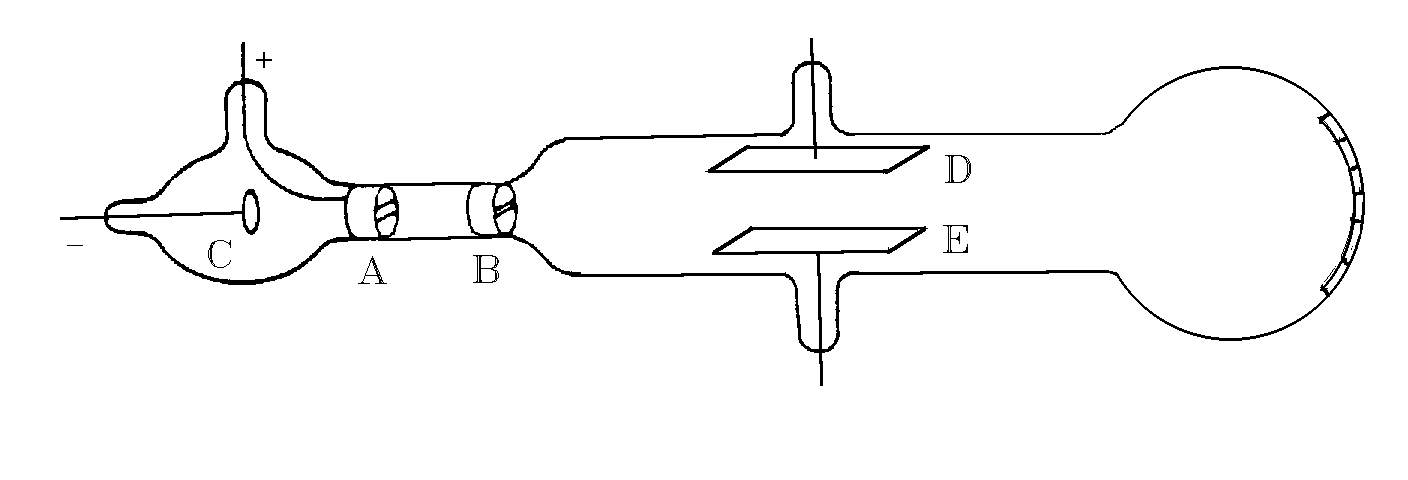
\includegraphics[width=4.32083in,height=1.94861in]{images/18_epr/image009.png}


The small body connected with the electron undergoes, however, a random
motion. Thus, it follows an irregular path starting out from point P, as
indicated in Fig. 3. Each electron then arrives at the screen at a
certain point. After a large number of electrons have passed through the
slit system, we will obtain a statistical pattern of such points, in
which the density of electrons is proportional to the field intensity, $|\psi|^2$ ,
at the screen. The statistical tendency to appear where $|\psi|^2$ is greatest is
due to the effects of the ``quantum-force'' while the random motions
explain why the precise points at which the various particles appear
fluctuate in an irregular way.

Now suppose that we close slit B. The wave pattern will now, as shown in
Fig. 4, cease to have strong and weak fringes. Thus, a new pattern of
electrons is obtained at the screen. Hence, the closing of slit B
influences even those particles that pass through slit A, because it
influences the ``quantum-force'' felt by the particle as it moves
between the slit system and the screen.

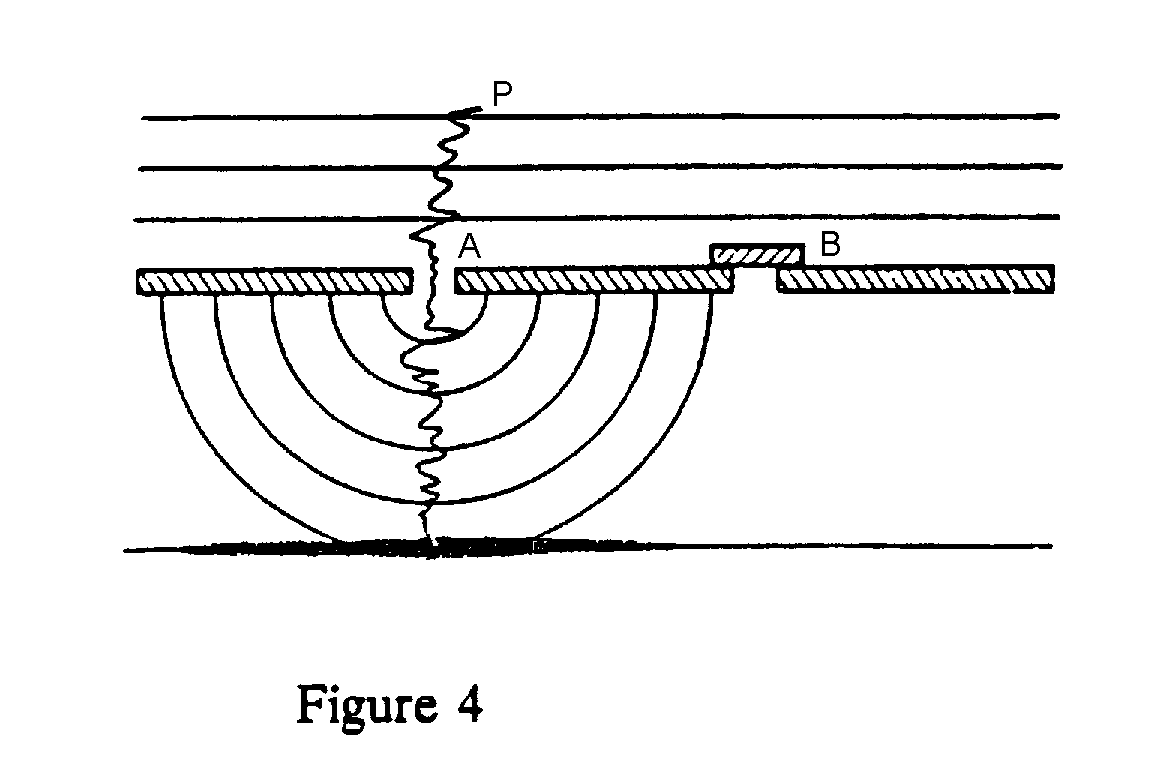
\includegraphics[width=4.60278in,height=3.08958in]{images/18_epr/image013.png}

In this way, we can understand how the wave-particle duality originates.
On the other hand, in the usual interpretation, no such an understanding
is possible. All that we can do is to accept without further discussion
the fact that electrons enter the slit system, and appear at the screen
with an interference pattern. As to how this came about, such a question
cannot even be raised within the framework of the usual interpretation.
\end{quote}

In two later articles\footnote{D. Bohm and B. Hiley, ``The de Broglie
  Pilot Wave Theory and the Further Development of New Insights Arising
  Out of It,'' \emph{Foundations of Physics} 12 (1982), 1001-10; D.
  Bohm, ``Hidden Variables and the Implicate Order'' in \emph{Quantum
  Implications}, B.J. Hiley and F.D. Peat, Edd. (London: Routledge \&
  Kegan Paul, 1987), 37-39.} Bohm presented his interpretation and
applied it to the EPR argument as follows:

\begin{quote}
Originally, Schrödinger regarded the wave intensity \ldots as the actual
density of electric charge, and this gave an image of the electron as a
unique and independent reality. However \ldots this assumed charge
density would spread out without limit in a short time; and yet, the
particle is always found in a small region of space. To resolve this
difficulty, Born proposed that the wave intensity is the probability
density of finding a particle. However, this left open the question of
whether the localized particle exists independently, or whether it is in
some sense produced or at least localized in the act of observation (as
is indeed implied in Heisenberg's analysis of the measurement of
position and momentum).

It is well-known that in the usual interpretation of the quantum theory,
the latter point of view is adopted.. The most consistent version of
this interpretation is that given by Bohr, in which no meaning can be
ascribed to precisely defined particle properties beyond the limits
specified by the Heisenberg uncertainty principle. This lack of meaning
goes beyond regarding these properties as independently existent, but
uncertain to us because of limits in our ability to obtain knowledge of
them through measurements. Rather, in Bohr's view, the universe is
basically an unanalyzable whole, in which the notion of the separateness
of particle and environment is an abstraction that has no content,
except as an approximation that may be applied within the limit of
Heisenberg's principle.

Most physicists have adopted views similar in key ways to those
described above, though the details vary considerably. However, de
Broglie, Ein\-stein, Schrö\-dinger, and others disagreed with this approach,
because they felt that there is a uniquely defined reality, which can be
grasped in thought and is yet independent of thought. Without
considering this reality, science is reduced to a set of formulas and
recipes for predicting the results of experiments. Indeed, a large
number of modern physicists have since then, at least tacitly, come to
adopt such a point of view, perhaps because it is part of the pragmatic
spirit of the age. However, in our view, this pragmatic approach is not
the only possible one, nor is it even the best. For one can see that
concepts that do not give immediate new experimental predictions may
still be valuable, in that they permit new insight and understanding
(from which new predictions may ultimately emerge). An approach that
discourages this kind of insight will thus tend to prevent creative new
perceptions, such as those of Einstein, de Broglie, etc.

The pilot wave theory of de Broglie was indeed a significant and
fruitful example of imaginative concepts that helped lead to new
insights\ldots.

In essence, de Broglie assumed that there is a physically real wave
satisfying Schrödinger's equation, at least as a linear approximation,
along with a particle following a well defined trajectory {[}and{]}
being ``guided'' by the background wave, and for this reason, de Broglie
called the latter a ``pilot wave.'' (One may here consider the analogy
of an airplane guided by radar waves, which carry information about the
whole environment.)\\
\centerline{* * *}

{[}Quantum mechanics implies{]} that each particle will be acted on, not
only by the classical potential, \emph{V}, but also by an additional
quantum potential \emph{Q}\ldots. In this interpretation, the new
features of quantum mechanics are seen to arise basically from \emph{Q.}

The first main difference {[}between classical and quantum mechanics{]}
can be seen by noting that the quantum potential, \emph{Q} \ldots{} does
not fall to zero at long distances, where the wave intensity becomes
negligible. However, the classical notion of analyzability of a system
into independent parts depends critically on the assumption that
whenever the parts are sufficiently far removed from each other, they do
not significantly interact. This means that the quantum theory implies a
new kind of wholeness, in which the behavior of a particle may depend
significantly on distant features of the over-all environment. This
dependence produces consequences similar to those implied by Bohr's
notion of unanalyzable wholeness, but different in that the universe can
be understood as a unique and in principle well defined reality.

To illustrate in more detail what is meant here, we consider an
interference experiment, in which a beam of electrons of definite
momentum is sent through a two slit system. In Fig. 5 we show the
results of a computation of the quantum potential\ldots.


\begin{center}
  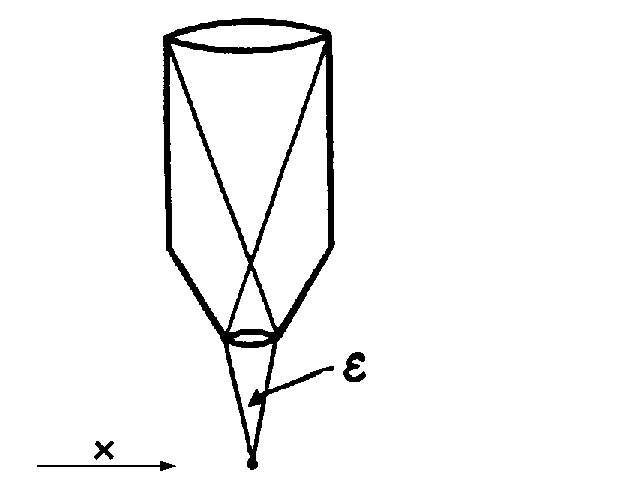
\includegraphics[width=2.21875in,height=3.13542in]{images/18_epr/image015.png}
\end{center}

What is especially significant in Fig. 5 is that the quantum potential
remains large at long distances from the slits, taking the form of a set
of valleys and high ridges, which latter gradually flatten out into
broad plateau\ldots. The fact that the quantum potential does not in
general fall off with the distance is thus what explains inter-ference
and diffraction patterns, and this is clearly
also what implies the kind of wholeness of particle and environment to which
we have referred above.


One may return here to the analogy of the airplane guided by radar
waves. Evidently, it is not a case of mechanical pressure of these waves
on the airplane, but rather, information concerning the whole
environment is enfolded by the waves, and carried into each region of
space. The airplane thus responds actively to the \emph{form} of the
waves, and this form is not altered as the intensity falls off with the
distance. A similar response to the \emph{form} of the quantum potential
is seen to be characteristic of the behavior of the electron. This means
that in the microworld, the concept of active information is relevant.

\centerline{* * *}

Thus, one could at least in principle have a strong and direct
(non-local) connection between particles that are quite distant from
each other. This sort of non-locality would, for example, give a simple
and direct explanation of the paradox of Einstein, Podolsky and Rosen,
because in measuring some property of one of a pair of particles with
correlated wave functions, one will alter the ``non-local'' quantum
potential so that the other particle responds in a corresponding way.

\centerline{* * *}

{[}W{]}hen the properties of the first particle are measured, the
quantum potential brings about a corresponding disturbance of the second
particle. And from this, it can be shown that in a statistical ensemble
of similar measurements, Heisenberg's uncer-tainty solutions \ldots will
still be obtained.

It follows then that with the aid of the quantum potential, something
like Heisenberg's original explanation of the uncertainty principle can
be maintained. The uncertainties in the properties of particles are
indeed now seen to follow from disturbances produced by the quantum
potential, whose effects are moreover unpredictable and uncontrollable,
because the current form of the theory is only able to provide
information concerning statistical distributions over the initial
conditions of all the particles concerned. (So that we cannot in
practice make observations of individual particles going beyond
Heisenberg's principle.)

\centerline{* * *}

{[}C{]}lassically, the whole is merely the result of the parts and their
pre-assigned interactions, so that the primary reality is the set of
parts while the behavior of the whole is derived entirely from those
parts and their interactions. With the quantum potential, however, the
whole has an independent and prior significance such that, indeed, the
whole may be said to organize the activities of the parts. For example,
in a superconducting state it may be seen that electrons are not
scattered because, through the action of the quantum potential, the
whole system is undergoing a coordinated movement more like a ballet
dance than like a crowd of unorganized people. Clearly, such quantum
wholeness of activity is closer to the organized unity of functioning of
the parts of a living being than it is to the kind of unity that is
obtained by putting together the parts of a machine.
\end{quote}
\end{document}
